\section{Post-selection inferens}
Klassisk statistisk inferens kan ikke anvendes for adaptive procedurer.
I dette afsnit beskrives en test til inferens efter variabeludvælgelse med en adaptiv metode.


\subsection{Kovarians test}
I dette afsnit introduceres en test der tildeler \(p\)-værdier til prediktorerne valgt af adaptive metoder.
Testen er baseret på LARS algoritmen og blev introduceret af \citep{lockhart}.

Betragt det velkendte lineær regression setup med en responsvariable \(\y \in \mathbb{R}^n\) og en matrix af prediktorer \(\X \in \mathbb{R}^{n \times p}\), relateret ved
\begin{align*}
\y = \X \beta + \boldsymbol{\epsilon}, \quad \boldsymbol{\epsilon} \sim N\del{\mathbf{0}, \sigma^2 \mathbf{I}_{n \times n}},
\end{align*}
hvor \(\beta \in \mathbb{R}^p\) er ukendte koefficienter som skal estimeres.

Lad $\lambda_1 > \lambda_2 > \ldots > \lambda_K$ være knuderne returneret af LARS algoritmen.
Disse er værdierne af regularitets parameteren $\lambda$ hvor der er en ændring i mængden af aktive prediktorer.
Antag vi ønsker, at teste om prediktoren valgt i \(\lambda_k\) fra LARS algoritmen er signifikant.
Lad \(\mathcal{A}_{k-1}\) være den aktive mængde, som består af prediktorerne med ikke-nul koefficienter, inden denne prediktor er tilføjet og lad estimatet til slut af dette trin være \(\hat{\beta} \del{\lambda_{k+1}}\).
Vi refitter lasso ved at lade \(\lambda=\lambda_{k+1}\) og blot at anvende variablerne i \(\mathcal{A}_{k-1}\).
Dette giver estimatet \( \hat{\beta}_{\mathcal{A}_{k-1}} \del{\lambda_{k+1}}\).
Kovarians teststørrelsen er defineret ved
\begin{align}
T_k = \frac{1}{\sigma^2} \del{ \left\langle \y, \X \hat{\beta} \del{\lambda_{k+1}} \right\rangle - \left\langle  \y, \X \hat{\beta}_{\mathcal{A}_{k-1}} \del{\lambda_{k+1}} \right\rangle}. \label{eq:6.5}
\end{align}
Teststørrelsen måler hvor stor en andel af kovariansen mellem outcome og den fittede model som kan tilskrives prediktoren som netop er tilføjet til modellen, dvs forbedringen over intervallet \(\del{\lambda_k, \lambda_{k+1}}\).

Under nulhypotesen at alle $k-1$ variable er i modellen, og under generelle betingelser for modelmatricen $\X$, gælder der for prediktoren i næste trin at
\begin{align*}
T_k \overset{d}{\rightarrow} \text{Exp}\del{1}
\end{align*}
når \(n, p \rightarrow \infty\).
Når \(\sigma^2\) er ukendt, kan den estimeres under den fulde model \(\hat{\sigma}^2 = \frac{1}{n-p} \text{RSS}_p\). 
Dette indsættes i \eqref{eq:6.5}, og eksponential testen bliver en eksakt \(F_{2,n-p}\) test.

Denne test erogså det naturlige analog til degrees of freedom resultaterne for lasso og LARS (section 2.5).
Lasso med \(k\) ikke-nul koefficienter forventes at have \(k\) frihedsgrader, og LARS anvender en frihedsgrad for hver segment \(\del{\lambda_{k+1}, \lambda_k}\) langs stien.
Kovarians testen har middelværdi lig en, som er antal frihedsgrader per trin.

\subsection{Teste baseret på polyhedral lemmaet}
\citep{post_inference}


I dette afsnit introduceres teste der er baseret på polyhedral lemmaet.
Testene er \textit{TG test} og \textit{spacing test}. 
Disse kan håndterer enhver procedure for hvilket udvægelsen kan karakteriseres ved en mængde af lineære uligheder i \(\y\).
Med andre ord kan udvægelsen skrives som \(\cbr{\mathbf{A} \y \leq b}\) for en matrix \(\mathbf{A}\) og vektor \(b\).
Den kan anvendes til trinene af LARS algoritmen, hvor det giver en eksakt form af kovarians testen.

Antag \(\y \sim N\del{\boldsymbol{\mu}, \sigma^2 \mathbf{I}_{n \times n}}\) og at vi ønsker at lave inferens betinget på hændelsen \(\cbr{\mathbf{A} \y \leq b}\).
Mere præcis ønsker vi at lave inferens om \(\boldsymbol{\eta}^T \boldsymbol{\mu}\), hvor \(\boldsymbol{\eta}\) muligvis afhænger af udvægelsen.
Hvis lasso, LARS .. har udvalgt denne mængde, da kan vi udføre inferens  af de udvalgte variable.
Vi kunne eventuelt være interesseret i regressions koefficienterne af \(\y\) på \(\X_\mathcal{A}\), dvs \(\hat{\theta}= \del{\X_\mathcal{A}^T \X_\mathcal{A}}^{-1} \X_\mathcal{A}^T \y\).
Disse svarer til populations parametrene \(\theta= \del{\X_\mathcal{A}^T \X_\mathcal{A}}^{-1} \X_\mathcal{A}^T \boldsymbol{\mu}\), koefficienterne af projectionen af \(\boldsymbol{\mu}\) på \(\X_\mathcal{A}\).
Dermed kunne \(\boldsymbol{\eta}^T \boldsymbol{\mu}\) svarer til én af disse koefficienter, og dermed er \(\boldsymbol{\eta}\) en af kolonnerne af \(\X_\mathcal{A} \del{\X_\mathcal{A}^T \X_\mathcal{A}}^{-1}\). Dette eksempel fortsættes senere.

\begin{lem}[Polyhedral lemma] \label{lem:polyhedral}
For ethvert \(\boldsymbol{\eta}\) hvor \(\Vert  \boldsymbol{\eta} \Vert_2^2 \neq 0\), da gælder, at
\begin{align}
\mathbf{A} \y \leq b \ \Longleftrightarrow \ \mathcal{V}^- \del{\y} \leq \boldsymbol{\eta}^T \y \leq \mathcal{V}^+ \del{\y}, \mathcal{V}^0 \del{\y} \leq 0, \label{eq:polyhedral}
\end{align}
hvor
\begin{align}
\mathcal{V}^- \del{\y} &= \max_{j: \alpha_j <0} \frac{b_j - \del{\mathbf{A} \y}_j + \alpha_j \boldsymbol{\eta}^T \y}{\alpha_j} \label{eq:V-} \\
\mathcal{V}^+ \del{\y} &= \min_{j: \alpha_j >0} \frac{b_j - \del{\mathbf{A} \y}_j + \alpha_j \boldsymbol{\eta}^T \y}{\alpha_j} \label{eq:V+} \\
\mathcal{V}^0 \del{\y} &= \min_{j: \alpha_j =0} \del{b_j - \del{\mathbf{A} \y}_j}.  \label{eq:V0} 
\end{align}
og \(\alpha=\frac{\mathbf{A} \boldsymbol{\eta}}{\Vert  \boldsymbol{\eta} \Vert_2^2}\).
Yderligere  er \(\boldsymbol{\eta}^T \y\) og \(\del{\mathcal{V}^-\del{\y}, \mathcal{V}^+\del{\y},\mathcal{V}^0\del{\y}}\) uafhængige. 
\end{lem}
\begin{proof}
Bevises undlades, men der henvises til --
\end{proof}
Resultatet i \eqref{eq:polyhedral} hvor \(\mathcal{V}^-\), \(\mathcal{V}^+\) og \(\mathcal{V}^0\) defineres i \eqref{eq:V-}-\eqref{eq:V0} er deterministisk og gælder for alle \(\y\).
Blot uafhængigheds resultatet afhænger af normaliteten af \(\y\).
Se figur -- for en geometrisk illustration af lemmaet.
Lad os dekomponere \(\y=P_{\boldsymbol{\eta}} \y + P_{\boldsymbol{\eta}^\perp} \y\), hvor \(P_{\boldsymbol{\eta}} \y = \frac{\boldsymbol{\eta} \boldsymbol{\eta}^T \y}{\Vert \boldsymbol{\eta} \Vert_2^2}\) er projectionen af \(\y\) langs \(\boldsymbol{\eta}\) og  \(P_{\boldsymbol{\eta}^\perp} \y = \y - P_{\boldsymbol{\eta}} \y\) er projectionen på orthokomplement af \(\boldsymbol{\eta}\).
Vi kan betragte \(\y\) som afvigelse fra \(P_{\boldsymbol{\eta}^\perp} \y\) af en mængde \(\boldsymbol{\eta}^T \y\), langs linjen bestemt af \(\boldsymbol{\eta}\).
Mængderne \(\mathcal{V}^-\) og \(\mathcal{V}^+\) betegner hvor langt vi kan afvige fra hver side af \(P_{\boldsymbol{\eta}^\perp} \y\) inden \(\y\) forlader polyhedronen.
Dette giver anledning til uligheden \(\mathcal{V}^- \leq \boldsymbol{\eta}^T \y \leq \mathcal{V}^+\).
Some faces of polyhedronen kan være perfekt justeret med \(\boldsymbol{\eta}\), dvs deres normal vektorer og \(\boldsymbol{\eta}\) er ortogonale.
Dette kan tjekkes udfra \(\mathcal{V}^0\) ved at \(\y\) ligger på den rigtige side af these faces.  

Betinget \(P_{\boldsymbol{\eta}^\perp} \y\), ses at hændelsen \(\cbr{\mathbf{A} \y \leq b}\) er ækvivalent med hændelsen \(\mathcal{V}^- \del{\y} \leq \boldsymbol{\eta}^T \y \leq \mathcal{V}^+ \del{\y}\). Yderligere er \(\mathcal{V}^- \del{\y}\) og \(\mathcal{V}^+ \del{\y}\) uafhængige af \(\boldsymbol{\eta}^T \y\), da disse kun er funktioner af \(P_{\boldsymbol{\eta}^\perp} \y\), som er uafhænige af \(\y\).


Af lemma \ref{lem:polyhedral} kan fordelingen af enhver lineær funktion \(\boldsymbol{\eta}^T \y\) betinget \(\mathbf{A} \y \leq b\) skrives som følgende betinget fordeling
\begin{align*}
\boldsymbol{\eta}^T \y \given \mathcal{V}^- \del{\y} \leq \boldsymbol{\eta}^T \y \leq \mathcal{V}^+ \del{\y}, \mathcal{V}^0 \del{\y} \leq 0.
\end{align*}
Da \(\boldsymbol{\eta}^T \y\) er normalfordelt, er overstående truncated normalfordelt, dvs med stokastiske truncation grænser.

\begin{figure}[H]
\centering
 \scalebox{0.7}{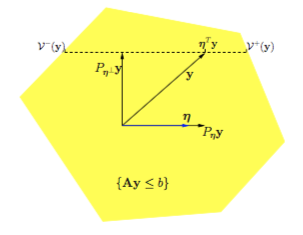
\includegraphics{fig/polyhedron.jpg}}
\caption{Geometrisk illstration af lemma \ref{lem:polyhedral} for \(n=2\) og \(\vert \boldsymbol{\eta} \Vert_2=1\). 
Det gule område er udvælgenses hændelsen \(\cbr{\mathbf{A} \y \leq b}\)}
\end{figure}


Vi definerer fordelingsfunktionen af en truncated normal fordeling med støtte begrænset af \(\sbr{c,d}\):
\begin{align*}
F_{\mu, \sigma^2}^{c,d} \del{x} = \frac{\Phi\del{\frac{x-\mu}{\sigma}} - \Phi\del{\frac{c-\mu}{\sigma}}}{\Phi\del{\frac{d-\mu}{\sigma}} - \Phi\del{\frac{c-\mu}{\sigma}}},
\end{align*}
hvor \(\Phi\) er fordelingsfunktionen af en standard normalfordeling.
Der gælder, at fordelingsfunktionen af en stokastisk variabel evalueret i værdien af denne variabel har en uniform fordeling. 
Derfor kan vi skrive, at
\begin{align}
F_{\boldsymbol{\eta}^T \boldsymbol{\mu}, \sigma^2 \Vert \boldsymbol{\eta} \Vert_2^2}^{\mathcal{V}^-, \mathcal{V}^+} \del{\boldsymbol{\eta}^T \y} \given \cbr{\mathbf{A} \y \leq b} \sim U \del{0,1}. \label{eq:6.10}
\end{align}
Heraf kan vi udlede testen. 
Lad os antage nulhypotesen
\begin{align*}
H_0: \boldsymbol{\eta}^T \boldsymbol{\mu}=0.
\end{align*}
Definer teststørrelsen
\begin{align}
T=2 \min\cbr{F_{0, \sigma^2 \Vert \boldsymbol{\eta} \Vert_2^2}^{\mathcal{V}^-, \mathcal{V}^+} \del{\boldsymbol{\eta}^T \y}, 1 - F_{0, \sigma^2 \Vert \boldsymbol{\eta} \Vert_2^2}^{\mathcal{V}^-, \mathcal{V}^+} \del{\boldsymbol{\eta}^T \y}}. \label{eq:m3.11}
\end{align}
Polyhedral lemmaet og teststørrelsen \eqref{eq:m3.11} kan anvendes som \(p\)-værdi for nulhypotensen $\boldsymbol{\eta}^T \boldsymbol{\mu}=0$ betinget \(\cbr{\mathbf{A} \y \leq 0}\).
For et signifikant niveau \(\alpha\) afvises nulhypotesen, hvis $T \leq \alpha$.

\subsubsection{TG test}
Herefter kan vi beskrive en test for lasso estimater som kan anvendes for ethvert \(\lambda\).

Vi definerer følgende teststørrelse
\begin{align*}
T^{\text{tg}}=1- F_{0, \sigma^2 \Vert \boldsymbol{\eta} \Vert_2^2}^{\mathcal{V}^-, \mathcal{V}^+} = \frac{\Phi \del{\frac{\mathcal{V}^+}{\sigma  \boldsymbol{\eta}^T  \boldsymbol{\eta}}}-\Phi \del{\frac{\boldsymbol{\eta}^T \y}{\sigma  \boldsymbol{\eta}^T  \boldsymbol{\eta}}}}{\Phi \del{\frac{\mathcal{V}^+}{\sigma  \boldsymbol{\eta}^T  \boldsymbol{\eta}}}-\Phi \del{\frac{\mathcal{V}^-}{\sigma  \boldsymbol{\eta}^T  \boldsymbol{\eta}}}}.
\end{align*}
Ifølge \eqref{eq:6.10} kan denne teststørrelse også anvendes som en \(p\)-værdi for \(H_0\) betinget \(\cbr{\mathbf{A} \y \leq 0}\).
For at teste \(H_0: \boldsymbol{\eta}^T \boldsymbol{\mu}=0\), er teststørrelsen
\begin{align*}
T^{\text{TG}}= 2 \min \cbr{T^{\text{tg}}, 1-T^{\text{tg}}}.
\end{align*}
For et signifikant niveau $\alpha$ afvises nulhypotesen hvis \(T^{\text{TG}} \leq \alpha\).

Herudfra kan vi også konstruere et betinget konfidens interval med konfidens niveau \(1-\alpha\).
Dette konfidens interval er givet ved \(\sbr{u_{\frac{\alpha}{2}}, u_{1-\frac{\alpha}{2}}}\), hvor grænserne opfylder
\begin{align*}
1-F_{u_{\frac{\alpha}{2}}, \sigma^2 \boldsymbol{\eta}^T  \boldsymbol{\eta} }^{\mathcal{V}^- \mathcal{V}^+} \del{\boldsymbol{\eta}^T \y} &= \frac{\alpha}{2} \\
1-F_{u_{1-\frac{\alpha}{2}}, \sigma^2 \boldsymbol{\eta}^T  \boldsymbol{\eta} }^{\mathcal{V}^- \mathcal{V}^+} \del{\boldsymbol{\eta}^T \y} &= 1-\frac{\alpha}{2}.
\end{align*}
Lad \(\mathcal{A}\) betegne den aktive mængde for et fast \(\lambda\) og lad \(\mathbf{e}_j\) være en \(p\)-dimensionel enhedsvektor.
Da kan vi teste om \(j\)'te variabel er signifikant, dvs \(H_0: \beta_j =0\), hvor \(\boldsymbol{\eta}=\del{\X_\mathcal{A}^+}^T \mathbf{e}_j\).
\begin{align*}
\boldsymbol{\eta}^T \boldsymbol{\mu} = \mathbf{e}_j^T \X_\mathcal{A}^+ \boldsymbol{\mu} = \mathbf{e}_j^T \del{\X^T \X}^{-1} \X^T \X \boldsymbol{\beta} = \beta_j.
\end{align*}
Nulhypotesen for TG testen er stokastisk, da \(\mathcal{V}^-\) og \(\mathcal{V}^+\) er stokastiske variable ...
TG testen for lasso antager blot en generel position af kolonnerne af \(\X\), som er en svag antagelse.
Testen kan bruges for ethvert fast \(\lambda\) og er eksakt.
%
\subsubsection{Spacing test}
Hvis variablen \(\mathbf{x}_{jk}\) vælges i det \(k\)'te trin i LARS algoritmen, da kan det vises at det tilhørende knude \(\lambda_k\) er givet ved \(\lambda_k = \boldsymbol{\eta}_k^T \y\) hvor
\begin{align*}
\boldsymbol{\eta}_k = \frac{\mathbf{P}^\perp_{\mathcal{A}_{k-1}} \mathbf{x}_{jk}}{s_k - \mathbf{x}_{jk}^T \X_{\mathcal{A}_{k-1}} \del{\X_{\mathcal{A}_{k-1}}^T \X_{\mathcal{A}_{k-1}}}^{-1} s_{\mathcal{A}_{k-1}}},
\end{align*}
hvor \(\mathcal{A}_{k-1}\) giver indeks af den aktive mængde efter \(k-1\) trin og
\begin{align*}
\mathbf{P}^\perp_{\mathcal{A}_{k-1}} = \mathbf{I}_n - \X_{\mathcal{A}_{k-1}} \del{\X_{\mathcal{A}_{k-1}}^T \X_{\mathcal{A}_{k-1}}}^{-1} \X _{\mathcal{A}_{k-1}}
\end{align*}
er residual projection operatoren som justerer \(\mathbf{x}_{jk}\) for \(\X_{\mathcal{A}_{k-1}}\).
Yderligere er \(s_k\) og \(s_{\mathcal{A}_{k-1}}\) fortegnene for koefficienterne for \(k\) variable som er indekseret ved \(\mathcal{A}_{k-1}\).

Matricen \(\mathbf{A}\) i knude \(\lambda_k\) har flere rækker end i det faste \(\lambda\) tilfælde, da vi betinger på hele følgen \(\cbr{\lambda_\ell}_1^k\).
Alligevel er udregningerne håndterbare og vi kan udregne eksakte \(p\)-værdier og konfidens intervaller for de valgte variable, som i det faste \(\lambda\) tilfælde.

At teste nulhypotesen \(H_0: \boldsymbol{\eta}^T \boldsymbol{\mu} =0\) er hermed ækvivalent med at teste \(H_0: \mathbf{e}_j^T \X_\mathcal{A}^+ \boldsymbol{\mu}=\beta_{j \ell}=0\).
Spacing testen tester altså om den tilføjede variable i \(k\)'te trin af LARS algoritmen er signifikant.
Vi definerer teststørrelsen
\begin{align*}
T_k^{\text{SP}}= \frac{\Phi \del{\lambda_{k-1} \frac{F \del{\mathcal{A}_{k-1}, s_{\mathcal{A}_{k-1}}, j}}{\sigma}} - \Phi \del{\lambda_{k} \frac{F \del{\mathcal{A}_{k-1}, s_{\mathcal{A}_{k-1}}, j}}{\sigma}}}{\Phi \del{\lambda_{k-1} \frac{F \del{\mathcal{A}_{k-1}, s_{\mathcal{A}_{k-1}}, j}}{\sigma}} - \Phi \del{M_{k}^+ \frac{F \del{\mathcal{A}_{k-1}, s_{\mathcal{A}_{k-1}}, j}}{\sigma}}}
\end{align*}
